%%%%%%%%%%%%%%
% Fichero: uclmTFGesi.tex
% Autor: Jesús Salido Tercero (http://www.uclm.es/profesorado/jsalido)
% Fecha (creación): Febrero 2010 
% Rev. : Febrero 2019
% Descripción: Plantilla para memoria de TFG 
% (Escuela Sup. de Informática, UCLM). Creada para el curso 
% “LaTeX esencial para preparación de TFG, Tesis y otros documentos 
% académicos” (Esc. Sup. Informática-UCLM)
%
% Comentarios: Preparada para `pdflatex' y `biblatex' (con `biber'). 
% Documento editado con TeXstudio. 
% Para su compilación se aconseja utilizar latexmk y biber (requiere perl):
% $latexmk -pdf -silent -synctex=1 --enable-write18 % (última opción innecesaria en Unix)
% En sistemas Unix: latexmk y biber deben ser instalados por separado.
%
% Una versión actualizada de esta plantilla está disponible en overleaf.
% Puede crearse un proyecto propio para escribir un TFG directamente en overleaf,
% o bien descargarla como un archivo .zip para su utilización en modo local.
%%%%%%%%%%%%%%


% -------------------------
%
% PREÁMBULO del documento
% (Editar sólo en caso de cambio del idioma pral. del documento u
%  opciones de los paquetes incluidos).
%
% -------------------------
% EDITAR: Idioma pral. \spanishtrue (Español), \spanishfalse (Inglés)
%Comentar opción no deseada
\newif\ifspanish%Definición de un condicional (spanish)

\spanishtrue 			% Idioma pral.: español (spanish=true)
%\spanishfalse			% Idioma pral.: inglés (spanish=false)
	
\documentclass[ 		% Clase del documento
	11pt,				% Tamaño de letra
	a4paper,			% Tamaño de papel
	twoside,			% Impresión a doble cara
	openright,			% La apertura de cap. a la dcha.
	final       		% Versión final
]{book}

\usepackage[utf8]{inputenx} % Codificación de entrada
\usepackage[english,spanish,es-tabla,es-noindentfirst]{babel} % Internacionalización
%\usepackage{indentfirst} % Para asegurar sangrado en 1ª línea tras sección (necesario con varios idiomas)

%--- Geometría de las páginas del documento
\usepackage[			% Márgenes del documento
	top=2.5cm,			% Margen superior
	bottom=2.5cm,		% Margen inferior
	inner=3.5cm,		% Margen al interior
	outer=2cm			% Margen al exterior
]{geometry}


%--- Tipografía
\usepackage{textcomp,marvosym,pifont} % Generación de símbolos especiales
\usepackage{ccicons} % Iconos de licencia Creative Commons
\usepackage{amsmath,amsthm,amssymb}	% Mejoras cuando hay matemáticas


%--- Tipografía (Opción 1)
\usepackage[tt=false]{libertine}	% Libertine
\usepackage[libertine]{newtxmath}	% Times
%---


%--- Tipografía (Opción 2)
%\usepackage{newpxtext}				% Palatino: La opción osf proporciona números en old style.
%\usepackage{newpxmath}				% Palatino
%---


\usepackage[T1]{fontenc}% Codificación de salida    
\usepackage{microtype}	% Mejoras de microtipografía en la obtención de PDF (sólo para pdflatex)


\usepackage{url} 		% Para escritura de URL
\urlstyle{sf}			% Estilo sans serif para URLs


%--- Definición de colores
% Este paquete debe cargarse antes de ctable.
% Revisar la documentación del paquete para ver los nombres de colores predefinidos.
\usepackage[%
	usenames,
	dvipsnames,
	svgnames,
	x11names,
	table
]{xcolor}


%--- Color especial definido para los hiperenlaces
\definecolor{palered}{rgb}{.8,0,0}


%--- Generación de hiperenlaces
\usepackage[
	pdftex,
	breaklinks,			% Permite que los links ocupen más de una línea
%	hidelinks,			% Oculta el color y borde de los links
% OJO: La opción colorlinks se comenta para evitar un error con el paquete menukeys. 
%	colorlinks=true,	% Pone color en los link o un borde
	linkcolor=palered,	% Color de los links
	anchorcolor=palered, 
	citecolor=palered, 
	filecolor=palered, 
	menucolor=palered, 
	urlcolor=palered,
	bookmarksnumbered=true % Incluye números en bookmarks
]{hyperref}


\usepackage{pdfpages}  % Permite inclusión de páginas de un PDF


%--- Paquetes para listas y organización de texto
\usepackage{paralist}	% Mayor control de listas
\usepackage{multicol}	% Texto en varias columnas


%--- Gráficos y tablas
\usepackage{graphicx}	% Inclusión de figuras
\usepackage{subfigure}	% Inclusión de subfiguras
% EDITAR: Si es necesario cambiar el path para los directorios de figuras.
\graphicspath{{./figs/}}% Path de búsqueda de ficheros gráficos
\DeclareGraphicsExtensions{.pdf,.png,.jpg} % Precedencia de extensiones
\usepackage{rotating}	% Giro de cajas (texto, figuras, tablas) (No DVI)
\usepackage{tabularx,booktabs}	% Ajustes para tablas


%--- Paquetes especiales para Informática
\usepackage{listings}	% Inclusión de listados de código

% Inclusión de algoritmos
\usepackage[
	lined,
	boxruled,
	algochapter,
	commentsnumbered,
\ifspanish
	spanish
\else
	english
\fi
]{algorithm2e}



%--- Personalización de títulos de figuras y tablas
\usepackage[%
	margin=10pt,		% Margen
	font=small,			% Tamaño de tipografía
	labelfont=bf,		% Prefijo-Etiqueta en negrita
	format=hang			%
]{caption}
\captionsetup[table]{skip=4pt} 	% Separación del caption en las tablas


%--- Bibliografía: Biblatex con biber.
% OJO: Para bib multilingüe añadir campos language y langid en registros bib.
\usepackage[
	backend=biber, 		% Backend
	sortcites,
	defernumbers=true, 	% Para numerar al final
	style=numeric-comp, % Estilo numérico condensado
%    style=apa,
%    citestyle=apa,
	% Descomentar las opciones siguientes para bibliografía multilingüe
%	autolang=other, 	% Requerido para opción multilingüe
%	language=auto   	% Requerido para opción multilingüe
]{biblatex}


% Línea añadida para eliminar el idioma de la fuente bibliográfica.
\AtEveryBibitem{\clearfield{note} \clearlist{language}}
% OJO: Editar si se cambia el fichero de bibliografía. 
\addbibresource{biblioTFG.bib} 	% Fichero de bibliografía.
\usepackage[autostyle]{csquotes}
%\DeclareLanguageMapping{spanish}{spanish-apa}
%---

\usepackage{float}
\usepackage[section]{placeins}

%--- Paquete con personalización local para el TFG (ESI-UCLM)
\usepackage{uclmTFGesi}
% -------------------------
% PAQUETES QUE USA: 
% 	fancyhdr,titlesec,sectsty,tikz
% -------------------------
% LISTA DE COMANDOS PROPORCIONADOS:
% OB-Obligatorio
% OP-Opcional
% RE-Recomendado
%
% Comandos para definir variables con los datos del documento.
%
% OB-\portadaTFG				: Pág. de portada (usa variables definidas)
% OB-\portadillaTFG				: Pág. de portada interna
% OB-\tribunalTFG				: Pág. tribunal
% RE-\dedicado{texto}			: Pág. de dedicatoria con texto
% RE-\creditos{texto}{imagen}	: Pág. de créditos con el texto y la imagen
% OB-\abstract{texto}			: Añade abstract (no definido en clase book)
% OP-\tecla{texto}				: Borde de tecla en torno al texto (sustituir por menukeys)		
% OP-\nodivide[penalty]			: Penaliza la división de palabras. 
%								  Máx. (n=10000) sin arg.
% OP-\nowidowandorphan[penalty]: Penaliza las viudas y huérfanas.
%								(sólo si necesario)
% OP-\nodividenotes[penalty]	: Penaliza la división de notas al pié 
%								entre págs.	(sólo si necesario)	
% OP-\savepagecnt				: Crea contador interno con el nº de pág. actual
% OP-\contpagination			: Recupera el valor de pág. previamente
%								 salvado en el cont. interno.
% RE-\cleanhdfirst				: Elimina la cabecera en la primera 
%								página de capítulo.
%
% -------------------------




%--- Paquete para índice temático
\usepackage{makeidx}
\makeindex


%--- Paquete para incluir menús, paths y teclas de modo "elegante"
% OJO: Este paquete presenta algunas incompatibilidades, debe cargarse el último y exige la desactivación de la opción colorlinks y la inclusión en este paquete de la opción hyperrefcolorlinks.
% Este paquete presenta alguna incompatibilidades por lo que cambiarlo de ubicación puede generar algún error (manejar con cuidado).
\usepackage[os=win,hyperrefcolorlinks]{menukeys}

% Estas definiciones permiten cambiar el estilo de los elementos. Si se desean otros estilos o su configuación es preciso recurrir a la documentación del paquete (no lo recomiendo).
\renewmenumacro{\menu}[>]{menus} % default: menus
\renewmenumacro{\directory}[/]{pathswithblackfolder} % default: paths
\renewmenumacro{\keys}[+]{shadowedroundedkeys} % default: roundedkeys

%%%%%%%%%%%%%%%%%%%%%%%%%%%%%%%%%%%%%%%%%%%%%%%%%%%%%
%%%%%%%%%%%%%%%%%%%%%%%%%%%%%%%%%%%%%%%%%%%%%%%%%%%%%
%%%%%%%%%%%%%%%%%%%%%%%%%%%%%%%%%%%%%%%%%%%%%%%%%%%%%

%--- Paquete para añadir celdas que combinen filas a tablas
\usepackage{multirow}



% -------------------------
%
% DATOS DEL DOCUMENTO 
% Definición de variables empleadas en el documento por lo que no son
% traducidos. Cuando algún campo puede tener varias líneas aparecen dos
% campos señalados como <campo>Primera y <campo>Segunda.
% Si no se desea emplear un campo este debe comentarse.
%
% -------------------------
% EDITAR: Datos del documento
\tituloPrimera{Diseño de un sistema de control de riego automatizado}	% 1ª Línea
\tituloSegunda{Aplicado a la viticultura}			% 2ª Línea  % Comentar si no existe
\titulo{Diseño de un sistema de control de riego automatizado}							% Título corto
\autor{Cristina Bolaños Peño}
\email{Cristina.Bolanos@alu.uclm.es}					
\director{Félix Jesús Villanueva Molina}
%\codirector{<codirector (nombre apellidos)>}	% Comentar si no existe
\instEdu{UNIVERSIDAD DE CASTILLA-LA MANCHA}
% Fichero con escudo de la institución
% Poner el logo del centro que corresponda
%\escudo{esi} 								
%\escudo{esicolor} 
%\escudo{logo_ESI} 							
\escudo{escudoInf} 	% Nucleo de ferrita						
%\escudo{uclm} 
%\escudo{etsii} 

\centroEdu{ESCUELA SUPERIOR DE INFORMÁTICA}
\deptoEduPrimera{Tecnologías y Sistemas de la Información}% 1ª Línea
%\deptoEduSegunda{<Segunda línea Depto. Director>}% 2ª Línea  % Comentar si no existe
\titulacion{GRADO EN INGENIERÍA INFORMÁTICA}
\especialidad{Ingeniería de Computadores} 			% Tecnología específica, ...
\tipoDoc{TRABAJO FIN DE GRADO}
% Si las fechas se desean en inglés hay que ponerlas explícitamente.
\fechaDef{junio, 2019} 							% Fecha de defensa
\mesDef{junio}        							% Mes de defensa
\yearDef{2019}        							% Año de defensa
\lugarDef{Ciudad Real}							% Lugar de defensa


% --- Propiedades para el documento PDF
\hypersetup{%
% EDITAR: Valores para el PDF.	
	pdftitle={Diseño de un sistema de control de riego automatizado}, 	% Título
	pdfauthor={C. Bolanos},	% Autor
	pdfsubject={Trabajo de Fin de Grado},	% Tema
	pdftoolbar=true,		% Muestra la toolbar de Acrobat
	pdfmenubar=true			% Muestra la menubar de Acrobat
}
% -------------------------


% -------------------------
%
% CUERPO DEL DOCUMENTO
%
% -------------------------
\begin{document}
	
%--- Ajustes del documento (en páginas iniciales).
\ifspanish
	\selectlanguage{spanish}% Emplea idioma español
\else
	\selectlanguage{english}% Emplea idioma inglés
\fi

\frontmatter
% Cambia la numeración de páginas a números romanos y las secciones no están numeradas aunque si aparecen en el índice de contenidos.
\pagestyle{empty}  % Páginas sin cabecera ni pies
%---



% -------------------------
%
% PORTADAS
%
% -------------------------
\portadaTFG		% Portada pral.

\portadillaTFG	% Portada interior (añade tutores)
%---






% -------------------------
%
% CRÉDITOS
%
% -------------------------
% EDITAR (opcional): Licencia (si se desea modificar).
% Este comando permite una gran flexibilidad y la ventaja de no depender de paquetes externos.
% Esta es una página reservada para señalar información relativa a los derechos de autor y la licencia de distribución y uso del documento. Esta página debería ser aprovechada también para informar de cualquier tipo de cesión de los derechos anteriormente citados. El autor del TFG debe tener presente que el incumplimiento de la legislación vigente en materia de protección de la propiedad intelectual es de su exclusiva responsabilidad independientemente de la cesión de derechos que este haya convenido para su obra ya que no son objeto de cesión aquellos derechos de los que no se es poseedor.

\creditos{Este documento se distribuye con licencia Creative Commons Atribución Compartir Igual 4.0. El texto completo de la licencia puede obtenerse en \url{https://creativecommons.org/licenses/by-sa/4.0/}. 
% El escudo de Informática basado en el nuclo de ferrita que acompaña la distribución de esta plantilla ha sido realizado por P.~Moya, D.~Villa e I. Díez, su inclusión debe respetar los derechos de autor y las licencias a las que se vea sometido. 

La copia y distribución de esta obra está permitida en todo el mundo, sin regalías y por cualquier medio, siempre que esta nota sea preservada. Se concede permiso para copiar y distribuir traducciones de este libro desde el español original a otro idioma, siempre que la traducción sea aprobada por el autor del libro y tanto el aviso de copyright como esta nota de permiso, sean preservados en todas las copias.}{cclicense}
%---




% -------------------------
%
% TRIBUNAL
%
% -------------------------
\tribunalTFG % Página para calificaciones del tribunal
%---





% -------------------------
%
% DEDICATORIA (opcional, 1 pág. máximo)
% Aunque opcional, no se debería perder la oportunidad de poder 
% dedicar el trabajo a alguien MUY especial.
%
% -------------------------
% EDITAR: Dedicatoria (comentar si no se desea incluir).
\dedicado{A toda mi familia \\ % A alguien muy especial
%(para siempre)
} % Como mucho dos líneas (no confundir con los agradecimientos).
%---









%--- Ajustes del documento.
\pagestyle{plain}	% Páginas sólo con numeración inferior al pie

% -------------------------
%
% RESUMEN:
% OJO: Si es preciso cambiar orden manualmente
%
% -------------------------
%--- Resumen en español
\selectlanguage{spanish} % Selección de idioma del resumen.
\cleardoublepage % Se incluye para modificar el contador de página antes de añadir bookmark
\phantomsection  % OJO: Necesario con hyperref
\pdfbookmark[0]{Resumen}{idx_resumen}% idx_resumen.0 % Bookmark en PDF


\begin{abstract}
% EDITAR: Resumen (máx. 1 pág.)
%\begin{center}
%\emph{(... versión del resumen en español ...)}
%\end{center}
La producción de productos agrícolas se ve afectada por desastres medio ambientales visibles en la actualidad, como lo son el calentamiento global, la contaminación o la deforestación. A esto hay que sumarle un mal uso de los recursos hídricos disponibles a nuestro alcance, sobretodo en el caso de grandes áreas de explotación. El clima mediterráneo del que presumía Castilla-La Mancha está al borde de la extinción y, por ello, la forma de cultivo debe volverse más eficiente.

Con este proyecto, se propone una nueva forma inteligente de gestionar el riego de plantaciones de medio o gran tamaño. De esta forma, se ha diseñado un sistema de sensores y actuadores que colaboran con los servicios en la nube para proporcionar al usuario agricultor un asistente en el empleo de agua.
\end{abstract}
%---










%--- Resumen en inglés
% Abstract
\selectlanguage{english} % Selección de idioma del resumen.
\cleardoublepage
\phantomsection % OJO: Necesario con hyperref
\pdfbookmark[0]{Abstract}{idx_abstract}% idx_abstract.0 % Bookmark en PDF

\begin{abstract}
% EDITAR: Abstract (máx. 1 pág.)

%\begin{center}
%\emph{(... english version of the abstract ...)}
%\end{center}
Farming production is affected by currently visible environmental problems, such as global warming, pollution or deforestation. Furthermore, an incorrect use of water resources can be as harmful as the mentioned, mostly on wider produciton areas.

Along this project, a new and smart form of irrigation on mean or large areas is discussed. With a series of sensors and actuators which communicates with Cloud Services, the farmer can be assisted on a efficiently use of water.
\end{abstract}
%---














% Selección de idioma para el resto del documento y adaptación de títulos de sección.
% EDITAR: Sólo si es necesario.
% NOTA: Al cambiar de idioma las def. de títulos se reinician.
\ifspanish
	\selectlanguage{spanish}% Para el resto del documento el idioma es español.
	%--- No necesarios al añadir la opción es-tabla para babel.
	%\renewcommand{\tablename}{Tabla} % Se sustituye 'Cuadro' por 'Tabla'
	%\renewcommand{\listtablename}{Índice de tablas}
	%---
	\renewcommand{\lstlistingname}{Listado}
	\renewcommand{\lstlistlistingname}{Índice de listados}
	\SetAlgorithmName{Algoritmo}{Alg}{Índice de algoritmos}
	% Modififica las macros \algorithmcfname y \listalgoritmcfname
	\renewcommand{\appendixname}{Anexo}
	\renewcommand{\bibname}{Bibliografía}
	\renewcommand{\indexname}{Índice temático}
\else
	\selectlanguage{english}
\fi

% -------------------------
%
% AGRADECIMIENTOS (recomendable máx. 1 pág.)
%
% -------------------------
\cleardoublepage
\phantomsection % OJO: Necesario con hyperref
\pdfbookmark[0]{Agradecimientos}{idx_agrad}% idx_agrad.0 % Bookmark en PDF

\chapter*{Agradecimientos} % Opción con * para que no aparezca en TOC ni numerada



\makeatletter		
\begin{flushright}
	\textit{\@autor}
\end{flushright}
\makeatother % Agradecimientos etc.












% -------------------------
%
% ÍNDICES
%
% -------------------------
\pagestyle{fancy} % Estilo de página ajustado por fancyhdr

% EDITAR: Si alguno de los índices no existe, su inclusión se puede comentar.
\cleardoublepage
\phantomsection % OJO: Necesario con hyperref
\pdfbookmark[0]{Índice general}{idx_toc}% idx_toc.0 % Bookmark en PDF

\tableofcontents  % Índice general

% Todos los listados se han incluido en el índice de contenidos. De modo automático también quedan añadidos a los bookmarks del PDF. Si se desean eliminiar del TOC se pueden comentar el comando \addcontensline.

\cleardoublepage
\phantomsection % OJO: Necesario con hyperref
\addcontentsline{toc}{chapter}{\listfigurename} % Añade la lista de figuras al TOC (también a bookmarks en PDF)
%\pdfbookmark[0]{\listfigurename}{idx_lof}% idx_lof.0 % Bookmark en PDF
\listoffigures    % Índice de figuras (opcional)

\cleardoublepage
\phantomsection % OJO: Necesario con hyperref
\addcontentsline{toc}{chapter}{\listtablename} % Añade la lista de tablas al TOC (también a bookmarks en PDF)
%\pdfbookmark[0]{\listtablename}{idx_lot}% idx_lot.0 % Bookmark en PDF
\listoftables % Índice de tablas (opcional)

\cleardoublepage
\phantomsection % OJO: Necesario con hyperref
\addcontentsline{toc}{chapter}{\lstlistlistingname} % Añade la lista de listados al TOC (también a bookmarks en PDF)
%\pdfbookmark[0]{\lstlistlistingname}{idx_lol}% idx_lol.0 % Bookmark en PDF
\lstlistoflistings % Índice de listados creados con listings (opcional)

\cleardoublepage
\phantomsection % OJO: Necesario con hyperref
\addcontentsline{toc}{chapter}{\listalgorithmcfname} % Añade la lista de algoritmos al TOC (también a bookmarks en PDF)
%\pdfbookmark[0]{\listalgorithmcfname}{idx_loa}% idx_loa.0 % Bookmark en PDF
\listofalgorithms % Índice de algoritmos creados con algortihm2e





























%--- MAINMATTER
% Capítulos del documento
% Salva en un contador interno el nº de páginas actual
% Debe ir antes de \mainmatter (antes de que se reinicie el cnt page)
\savepagecnt
\mainmatter
% Justo antes del primer capítulo del libro. Activa la numeración con números arábigos y reinicia el contador de páginas.

% OJO: No cambiar de ubicación. Elimina cabecera y pie en pág. inicial de cap.
\cleanhdfirst

% Reajuste del número de página consecutivo para no reiniciar paginación en Cáp. 1
%\contpagination % Comentado para reiniciar paginación (pag. 1)




% -------------------------
%
% CAPÍTULOS
%
% -------------------------
% Se incluye un fichero para cada capítulo. Se emplea la instrucción \include porque en los libros lo más habitual es que cada cápítulo comience en una nueva página.

% OBLIGATORIOS: Motivacion, objetivos generales y específicos, metodología de trabajo, resultados, conclusiones
\chapter{Introducción}
\label{cap:Introduccion}

%   Definición del problema principal
Los desastres climáticos conforman una realidad sumamente atroz, la cual está presente en los medios de comunicación a día de hoy. Sin ir más lejos, en este 2019 se han organizando numerosas manifestaciones en todo el globo en forma de protesta contra la pasividad ante el cambio climático y concienciar a la población antes de llegar al 2030, el año de no retorno \cite{elpais01}.
% Recurso: Fotos Marchas 15: https://elpais.com/Comentario/1552688956-d7e20feb8fbbb828976c52707f1ea897?gla=es

Si no es uno de los más importantes, el calentamiento global acarreará una de las más catastróficas consecuencias, aunque hay muchas más: la falta de agua potable. Ésta marcará la supervivencia del ser humano, pues no sólo escaseará en el consumo directo, si no en la producción de bienes agrícolas y ganaderos. Acercándonos al campo de la agricultura, sólo en Castilla-La Mancha se emplearon 1.655.033 miles de metros cúbicos de agua en 2016 \cite{ine01}.

%   Soluciones actuales
Las soluciones a la escasez hídrica radican en el empleo de un sistema de riego adecuado al cultivo y tamaño de este. Nos encontramos, de entre todas ellas, dos destacadas: la aspersión y el goteo. Sin embargo, de entre todas estas alternativas, ninguna aporta una solución eficaz en relación al entorno que rodea al terreno, y si lo hacen, sólo pueden aplicarse a zonas de menor tamaño y con mayor control del sus condiciones, como podrían ser invernaderos.

%   Solución obtenida
La tecnología del \emph{Internet de las Cosas}, referido de ahora en adelante como IoT, permite parametrizar situaciones que vivimos diariamente y nos da la posibilidad de actuar frente a posibles cambios en esos datos en un tiempo mínimo. Algunos ejemplos son las ciudades inteligentes o la conectividad entre vehículos.

A lo largo de este proyecto se desarrollará la idea de un sistema IoT de agricultura inteligente, el cual recogerá datos del propio cultivo relativos al crecimiento y cuidado del mismo y posteriormente se analizarán para su debida reacción en el suministro de agua. Con ella, se podrá optimizar el ciclo de riego de la producción con datos que proporciona el mismo y reaccionar ante ellos de forma casi instantánea.

El objetivo principal del proyecto es la reducción de la cantidad de recursos utilizados, ya sean hídricos o eléctricos (consumidos al extraer u obtener los primeros) a la par que se optimiza el ciclo de vida del cultivo proporcionando al cultivo agua únicamente y siempre en el momento en el que lo necesite. Al agricultor se le facilitará una herramienta donde tendrá centralizados todos los terrenos de los que disponga y podrá visualizar el estado de cada uno en tiempo real y desde cualquier plataforma. 
\chapter{Objetivo}
\label{cap:Objetivo}

En el siguiente capítulo se detallará al lector la finalidad de este Trabajo de Fin de Carrera, en adelante referido como TFG, así como sus funcionalidades y objetivos más específicos.

\section{Objetivo general}
\label{sec:general}

El objetivo principal es el obtener un sistema de control de riego para cultivos de medio o mayor tamaño que informe al agricultor del estado del mismo, además de poder retroalimentarse de esa información y activar el riego en función de estos.

\section{Objetivos parciales}
\label{sec:especificos}

\subsection{Análisis de las arquitecturas y tecnologías de comunicación a utilizar}
\label{subsec:analisis_arquitecturas_tecnologias}

\subsection{Selección de sensores y módulos de comunicaciones de IoT}
\label{subsec:seleccion_sensores}

\subsection{Implementación de software de recolección de datos de los sensores}
\label{subsec:implementacion_recoleccion}

\subsection{Implementación de software de comunicación entre los nodos y la pasarela}
\label{subsec:implementacion_comunicacion_sublc}

\subsection{Implementación de software de comunicación entre el servicio en la nube y la pasarela}
\label{subsec:implementacion_comunicacion_subi}

\subsection{Implementación de software de monitorización de los datos recolectados}
\label{subsec:implementacion_monitorizacion}

\subsection{Implementación de software de actuación y/o reacción sobre el terreno}
\label{subsec:implementacion_actuacion}
\chapter{Metodología de trabajo}
\label{cap:Metodologia}

En este capítulo se detalla la metodología de trabajo empleada para lograr los objetivos marcados en el Capítulo \ref{cap:Objetivo}, así como en el desarrollo del proyecto  y las herramientas, tanto software como hardware, utilizadas en el mismo.

\section{Elección y breve descripción}
\label{sec:Elección}

Para la elaboración de este TFG se ha empleado el Proceso Unificado de Desarrollo, de ahora en adelante referido como PUD, como metodología de trabajo. Tal y como se define en \cite{PUD2017}:

\begin{quote}
    El PUD es un marco genérico que puede especializarse para una gran variedad de sistemas de software, para diferentes áreas de aplicación, diferentes tipos de organizaciones, diferentes niveles de aptitud y diferentes tamaños de proyectos.
\end{quote}

Se ha optado por dicha alternativa por su relativa sencillez, generalidad, y la amplitud de control de software que ofrece.

Para diseñar y realizar los modelos de cualquier sistema, PUD hace uso del Lenguaje Unificado de Modelado, en adelante referido como UML, el cual se ha utilizado en este proyecto en sus diferentes etapas. Cabe mencionar que el PUD se caracteriza por:
\begin{compactitem}
    \item Ser iterativo e incremental.
    \item Estar basado en la arquitectura.
    \item Estar dirigido por casos de uso.
\end{compactitem}

\section{Gestión del proyecto}
\label{sec:Gestion}

\subsection{Fases}
\label{subsec:Fases}

Siguiendo la estructura del ciclo de vida de un producto software definido por PUD, se han establecido las siguientes pautas o fases generales a seguir:

\begin{enumerate}
    \item \textbf{Inicio}: Se llevará a cabo una descripción del producto final que se desea conseguir, estudiando el alcance del proyecto, su viabilidad, y la planificación del desarrollo del proyecto. Se obtienen:
    \begin{enumerate}
        \item Modelo de casos de uso, el cual describe las funcionalidades del sistema.
    \end{enumerate}
    \item \textbf{Elaboración}: Se desarrollará y trabajará en el modelo obtenido en la fase anterior profundizando así en la arquitectura del sistema, consiguiendo la línea base de ésta. Se obtienen:
    \begin{enumerate}
        \item Modelo de análisis, con el que desarrollamos las funcionalidades en procesos, interfaces o bancos de datos.
        \item Modelo de diseño, obteniendo un despliegue mucho más especifico del modelo anterior.
    \end{enumerate}
    \item \textbf{Construcción}: Se implementará y probará el producto, tanto su despliegue físico como el software de cada uno de sus componentes. Se obtiene:
    \begin{enumerate}
        \item Modelo de implementación, con el que se conseguirá representar la ejecución total del sistema.
        \item Modelo de pruebas, el cual contiene el conjunto de casos de pruebas unitarias que se realizan al finalizar cada una de las fases del PUD.
    \end{enumerate}
    \item \textbf{Transición}: Al llegar a esta etapa, el producto está en su versión beta y se procede a la evaluación del mismo en busca de errores o deficiencias. Se obtiene:
    \begin{enumerate}
        \item Versión del producto final.
        \item Documentación del desarrollo.
    \end{enumerate}
\end{enumerate}

\subsection{Aplicación}
\label{subsec:Aplicacion}

En este apartado se muestra de qué manera se ha aplicado el PUD para la gestión del proyecto. Posteriormente, en el Capítulo \ref{cap:Resultados} se detallarán los artefactos resultantes de dicha aplicación para cada una de las iteraciones.

En la Tabla \ref{tab:iteraciones} se puede observar un resumen de la planificación del proyecto y de sus iteraciones. Para cada una de estas últimas se han aportado los objetivos más relevantes.

\begin{table}[htb]
    \centering
    \caption{Planificación de iteraciones}
    \label{tab:iteraciones}
    \begin{tabular}[t]{ | c | c | p{8cm} |}
         \hline
         \textbf{Fase} &  \textbf{Iteración} & \textbf{Objetivos}\\
         \hline\hline
         Inicio &  Preliminar & 
         Planificación del proyecto, estudio de su alcance y viabilidad, realizar el documento del Anteproyecto, captura de requisitos y modelado de casos de uso.\\
         \hline
         \multirow{2}{*}{Elaboración}
         & 1 & Definición de la arquitectura del sistema y modelado de casos de uso detallado.\\
         \cline{2-3}
         & 2 & Realizar el modelo de análisis y de diseño, preparación del entorno de desarrollo.\\
         \hline\multirow{6}{*}{Construcción}
         & 3 & Desarrollo de las funcionalidades que engloba CdU.01 Acceso/Registro.\\
         \cline{2-3}
         & 4 & Desarrollo de las funcionalidades que engloba CdU.02 Visualización\\
         \cline{2-3}
         & 5 & Desarrollo de las funcionalidades que engloba CdU.03 Gestión de configuración\\
         \cline{2-3}
         & 6 & Desarrollo de las funcionalidades que engloba CdU.04 Recolección de información\\
         \cline{2-3}
         & 7 & Desarrollo de las funcionalidades que engloba CdU.05 Aplicación de comandos\\
         \hline
         \multirow{3}{*}{Transición}
         & 8 & Despliegue del sistema.\\
         \cline{2-3}
         & 9 & Pruebas.\\
         \cline{2-3}
         & 10 & Documentación del proyecto y manual de usuario.\\
         \hline
    \end{tabular}
\end{table}


\section{Marco tecnológico}
\label{sec:metodologia.herramientas}

\subsection{Herramientas hardware}
\label{subsec:metodologia.herramientas.hardware}

\begin{itemize}
    \item PyCom
    \item Módulo LoRa
    \item Ordenador del lab
    \item DHT22
    \item Sensor de tierra
\end{itemize}

\subsection{Herramientas para la gestión de proyectos}
\label{subsec:metodologia.herramientas.proyectos}

\begin{itemize}
    \item Bitbucket
    \item Mercurial
    \item Microsoft Project
    \item Métrica v.3
\end{itemize}

\subsection{Herramientas, lenguajes y tecnologías para el modelado de software}
\label{subsec:metodologia.herramientas.software.modelado}

\begin{itemize}
    \item Visual Paradigm
    \item UML
\end{itemize}

\subsection{Herramientas, lenguajes y tecnologías para el desarrollo de software}
\label{subsec:metodologia.herramientas.software.desarrollo}

\begin{itemize}
    \item Atom
    \item pymakr
    \item Python
    \item Micropython
\end{itemize}

\subsection{Herramientas para la elaboración de la documentación}
\label{subsec:metodologia.herramientas.documentacion}

\begin{itemize}
    \item \LaTeX
    \item Overleaf
    \item Draw.io
\end{itemize}

\begin{itemize}
    \item Docker --> Resultados
    \item MySql Server --> Resultados
    \item Grafana --> Resultados
\end{itemize}
\chapter{Resultados}
\label{cap:Resultados}

En esta sección se describirá la aplicación del método de trabajo presentado en el Capítulo \ref{cap:Metodologia} en este caso concreto, mostrando los elementos (modelos, diagramas, especificaciones, etc.) más importantes. Este apartado debe explicar cómo la metodología satisface los objetivos planteados en el Capítulo \ref{cap:Objetivo}.

\section{Fase de Inicio}
\label{sec:Resultados.Inicio}

En dicha fase tiene lugar una única iteración, como podemos comprobar en la tabla \ref{tab:iteraciones}. En esta etapa del ciclo de vida del proyecto se llevará a cabo el estudio de viabilidad del mismo, la captura e identificación de los requisitos, y una planificación de sus iteraciones.

\subsection{Estudio de Viabilidad}
\label{subsec:Resultados.Inicio.Viabilidad}

\subsection{Captura de Requisitos}
\label{subsec:Resultados.Inicio.Requisitos}

Tras analizar los objetivos a conseguir descritos en el Capítulo \ref{cap:Objetivo} se analizaron las necesidades y funcionalidades que el sistema debía cumplir, además de considerar las posibles restricciones que afecten al proyecto. Hecho esto, se elaboró la siguiente lista de requisitos funcionales:

\begin{itemize}
    \item \textbf{RF.01 Acceso y/o Registro:}
    El usuario debe poder registrarse en el caso de que lo requiera y, por consiguiente, acceder al resto de funcionalidades del sistema.
    \item \textbf{RF.02 Monitorización del cultivo:}
    El usuario podrá visualizar los datos de su cultivo en tiempo real.
    \item \textbf{RF.03 Gestión de la configuración:}
    El usuario podrá gestionar su cultivo, cambiar sus datos así como los de él mismo.
    \item \textbf{RF.04 Recolección de información:}
    A través de sensores el sistema obtendrá información sobre el terreno.
    \item \textbf{RF.05 Envío de información:}
    Se enviará la información recogida a un servicio a través de la red.
    \item \textbf{RF.06 Análisis y Almacenamiento:}
    La información recogida se analizará para si el riego es o no suficiente en ese instante y se almacenará en una base de datos.
    \item \textbf{RF.07 Envío de acciones:}
    Se enviarán comandos a los dispositivos desplegados en el terreno a aplicar en el volumen de agua suministrado en función de si se ha determinado que el riego es o no suficiente.
    \item \textbf{RF.08 Recepción de comandos:}
    Los dispositivos desplegados en el terreno deben poder recibir los distintos comandos a aplicar a través de la red.
    \item \textbf{RF.09 Aplicación de comandos:}
    Los dispositivos desplegados en el terreno deben poder cambiar, aumentar o disminuir, el volumen de riego aplicado el terreno.
\end{itemize}

También se identificaron los siguientes requisitos no funcionales:

\begin{itemize}
    \item \textbf{RNF.01 Alojamiento en la nube:}
    El servicio en la red al que el usuario accederá debe estar alojado en algún servicio de alojamiento en la nube por la independencia de infraestructura y en libre acceso desde cualquier parte del mundo, además de proporcionar unos sistemas de seguridad básicos.
    \item \textbf{RNF.02 Comunicaciones de largo alcance:}
    Las comunicaciones que se empleen deben ser de largo alcance, ya sean inalámbricas o no, aunque por ello no debe aumentar excesivamente el coste del proyecto.
    \item \textbf{RNF.03 División en secciones:}
    El terreno, al ser una superficie grande, puede subdividirse en zonas más pequeñas para su correcta parametrización en el sistema.
    \item \textbf{RNF.04 Encriptación de mensajes:}
    Todos los datos que se envíen y reciban deben estar encriptados con un algoritmo adecuado para ello para asegurar definitivamente la no manipulación de los mismos.
\end{itemize}

\FloatBarrier
\subsection{Artefactos obtenidos}
\label{subsec:Resultados.Inicio.Artefactos}

Como artefactos resultantes de la finalización de esta fase, con la aplicación del PUD descrito en el Capítulo \ref{cap:Metodologia} y tras la identificación de los requisitos en la Sección \ref{subsec:Resultados.Inicio.Requisitos}, obtenemos una versión inicial del modelo de casos de uso del sistema.

Éstos se han obtenido tras a aplicar la trazabilidad de requisitos a casos de uso con uso del PUD. Partiendo de los requisitos anteriormente especificados, y de la suposición de que varios requisitos funcionales pueden proyectarse en un caso de uso, obtenemos los siguientes casos de uso:

\begin{table}[htb]
    \centering
    \caption{Trazabilidad de requisitos}
    \begin{tabular}[t]{ | r | l |}
        \hline
        \textbf{Caso de Uso} & \textbf{Requisito Funcional} \\ \hline \hline
        CdU.01 Acceso/Registro & RF.01 Acceso y/o Registro \\ \hline
        CdU.02 Visualización & RF.02 Monitorización del cultivo \\ \hline
        CdU.03 Gestión de configuración & RF.03 Gestión de la configuración \\ \hline
        \multirow{2}{*}{CdU.04 Recolección de información}
        & RF.04 Recolección de información \\
        & RF.05 Envío de información \\
        & RF.06 Análisis y Almacenamiento \\
        \hline
        \multirow{2}{*}{CdU.05 Aplicación de comandos}
        & RF.07 Envío de acciones \\
        & RF.08 Recepción de comandos \\
        & RF.09 Aplicación de comandos \\
        \hline
    \end{tabular}
    \label{tab:Trazabilidad.Requisitos}
\end{table}

En la figura \ref{fig:tfg-DCU-00} podemos observar el diagrama de casos de uso del sistema completo a un alto nivel de abstracción.

\begin{figure}[htb]
	\centering
	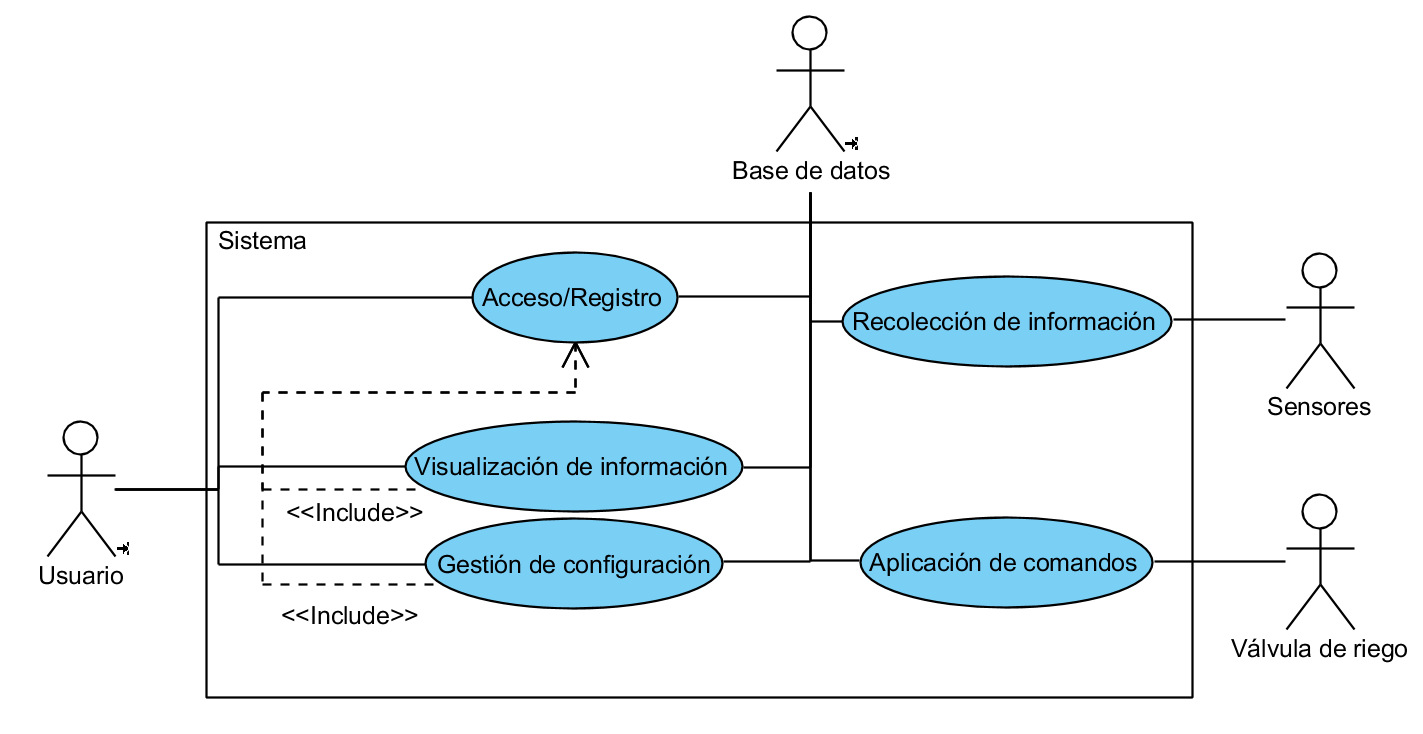
\includegraphics[width=0.80\textwidth]{figs/Modelos/tfg-DCU-00.png}
	\caption[Modelo de Casos de Uso Inicial]{Versión inicial del Modelo de Casos de Uso}
	\label{fig:tfg-DCU-00}
\end{figure}

\FloatBarrier
\subsection{Planificación de Iteraciones}
\label{subsec:Resultados.Inicio.Planificación}

Se ha llevado a cabo una planificación del proyecto con ayuda de la identificación de las distintas iteraciones a completar gracias a la herramienta de Microsoft project.

\begin{table}[hbt]
    \centering
    \caption{Iteración preliminar}
    \label{tab:resultados.planificacion.iter.pre}
    \begin{tabular}[t]{| l || p{8cm} |}
        \hline
        \textbf{Iteración} & Preliminar \\ \hline
        \textbf{Fase} & Inicio \\ \hline
        \multirow{1}{*}{\textbf{Objetivos}}
        & Captura de Requisitos \\ \cline{2-2}
        & Versión inicial del modelo de casos de uso \\ \cline{2-2}
        & Planificación del proyecto \\ \cline{2-2}
        & Estudio de viabilidad \\ \cline{2-2}
        & Anteproyecto aprobado por la comisión académica encargada de dicha tarea \\ \hline
        \multirow{1}{*}{\textbf{Artefactos}}
        & Requisitos funcionales y no funcionales del proyecto \\ \cline{2-2}
        & Diagrama de casos de uso \\ \cline{2-2}
        & Documento del Anteproyecto \\
        \hline
    \end{tabular}
\end{table}

\begin{table}[htb]
    \centering
    \caption{Iteración 1}
    \label{tab:resultados.planificacion.iter.1}
    \begin{tabular}[t]{| l || p{8cm} |}
        \hline
        \textbf{Iteración} & 1 \\ \hline
        \textbf{Fase} & Elaboración \\ \hline
        \multirow{1}{*}{\textbf{Objetivos}}
        & Modelo de casos de uso detallado \\ \cline{2-2}
        & Definición de la línea base de la arquitectura \\ \hline
        \multirow{1}{*}{\textbf{Artefactos}}
        & Segunda versión del diagrama de casos de uso \\ \cline{2-2}
        & Diseño de la arquitectura \\
        \hline
    \end{tabular}
\end{table}

\begin{table}[htb]
    \centering
    \caption{Iteración 2}
    \label{tab:resultados.planificacion.iter.2}
    \begin{tabular}[t]{| l || p{8cm} |}
        \hline
        \textbf{Iteración} & 2 \\ \hline
        \textbf{Fase} & Elaboración \\ \hline
        \multirow{1}{*}{\textbf{Objetivos}}
        & Modelo de análisis \\ \cline{2-2}
        & Modelo de diseño \\ \hline
        \multirow{1}{*}{\textbf{Artefactos}}
        & Diagrama de clases de análisis \\ \cline{2-2}
        & Diagrama de clases de diseño \\
        \hline
    \end{tabular}
\end{table}

\begin{table}[htb]
    \centering
    \caption{Iteración 3}
    \label{tab:resultados.planificacion.iter.3}
    \begin{tabular}[t]{| l || p{8cm} |}
        \hline
        \textbf{Iteración} & 3 \\ \hline
        \textbf{Fase} & Construcción \\ \hline
        \multirow{1}{*}{\textbf{Objetivos}}
        & Implementación del caso de uso CdU.01 \\ \cline{2-2}
        & Pruebas de integración \\ \hline
        \multirow{1}{*}{\textbf{Artefactos}}
        & Diagrama de secuencia del caso de uso CdU.01 \\ \cline{2-2}
        & Resultado de las pruebas \\
        \hline
    \end{tabular}
\end{table}

\begin{table}[htb]
    \centering
    \caption{Iteración 4}
    \label{tab:resultados.planificacion.iter.4}
    \begin{tabular}[t]{| l || p{8cm} |}
        \hline
        \textbf{Iteración} & 4 \\ \hline
        \textbf{Fase} & Construcción \\ \hline
        \multirow{1}{*}{\textbf{Objetivos}}
        & Implementación del caso de uso CdU.02 \\ \cline{2-2}
        & Pruebas de integración \\ \hline
        \multirow{1}{*}{\textbf{Artefactos}}
        & Diagrama de secuencia del caso de uso CdU.02 \\ \cline{2-2}
        & Resultado de las pruebas \\
        \hline
    \end{tabular}
\end{table}

\begin{table}[htb]
    \centering
    \caption{Iteración 5}
    \label{tab:resultados.planificacion.iter.5}
    \begin{tabular}[t]{| l || p{8cm} |}
        \hline
        \textbf{Iteración} & 5 \\ \hline
        \textbf{Fase} & Construcción \\ \hline
        \multirow{1}{*}{\textbf{Objetivos}}
        & Implementación del caso de uso CdU.03 \\ \cline{2-2}
        & Pruebas de integración \\ \hline
        \multirow{1}{*}{\textbf{Artefactos}}
        & Diagrama de secuencia del caso de uso CdU.03 \\ \cline{2-2}
        & Resultado de las pruebas \\
        \hline
    \end{tabular}
\end{table}

\begin{table}[htb]
    \centering
    \caption{Iteración 6}
    \label{tab:resultados.planificacion.iter.6}
    \begin{tabular}[t]{| l || p{8cm} |}
        \hline
        \textbf{Iteración} & 6 \\ \hline
        \textbf{Fase} & Construcción \\ \hline
        \multirow{1}{*}{\textbf{Objetivos}}
        & Implementación del caso de uso CdU.04 \\ \cline{2-2}
        & Pruebas de integración \\ \hline
        \multirow{1}{*}{\textbf{Artefactos}}
        & Diagrama de secuencia del caso de uso CdU.04 \\ \cline{2-2}
        & Resultado de las pruebas \\
        \hline
    \end{tabular}
\end{table}

\begin{table}[htb]
    \centering
    \caption{Iteración 7}
    \label{tab:resultados.planificacion.iter.7}
    \begin{tabular}[t]{| l || p{8cm} |}
        \hline
        \textbf{Iteración} & 7 \\ \hline
        \textbf{Fase} & Construcción \\ \hline
        \multirow{1}{*}{\textbf{Objetivos}}
        & Implementación del caso de uso CdU.05 \\ \cline{2-2}
        & Pruebas de integración \\ \hline
        \multirow{1}{*}{\textbf{Artefactos}}
        & Diagrama de secuencia del caso de uso CdU.05 \\ \cline{2-2}
        & Resultado de las pruebas \\
        \hline
    \end{tabular}
\end{table}

\begin{table}[htb]
    \centering
    \caption{Iteración 8}
    \label{tab:resultados.planificacion.iter.8}
    \begin{tabular}[t]{| l || p{8cm} |}
        \hline
        \textbf{Iteración} & 8 \\ \hline
        \textbf{Fase} & Transición \\ \hline
        \multirow{1}{*}{\textbf{Objetivos}}
        & Despliegue del sistema completo \\ \hline
        \multirow{1}{*}{\textbf{Artefactos}}
        & Sistema desplegado y funcional \\
        \hline
    \end{tabular}
\end{table}

\begin{table}[htb]
    \centering
    \caption{Iteración 9}
    \label{tab:resultados.planificacion.iter.9}
    \begin{tabular}[t]{| l || p{8cm} |}
        \hline
        \textbf{Iteración} & 9 \\ \hline
        \textbf{Fase} & Transición \\ \hline
        \multirow{1}{*}{\textbf{Objetivos}}
        & Realización de pruebas en el sistema desplegado \\ \hline
        \multirow{1}{*}{\textbf{Artefactos}}
        & Resultados de las pruebas \\
        \hline
    \end{tabular}
\end{table}

\begin{table}[htb]
    \centering
    \caption{Iteración 10}
    \label{tab:resultados.planificacion.iter.10}
    \begin{tabular}[t]{| l || p{8cm} |}
        \hline
        \textbf{Iteración} & 10 \\ \hline
        \textbf{Fase} & Transición \\ \hline
        \multirow{1}{*}{\textbf{Objetivos}}
        & Documentación del proyecto \\ \cline{2-2}
        & Elaboración de los manuales de usuario correspondientes \\ \hline
        \multirow{1}{*}{\textbf{Artefactos}}
        & Memoria del TFG \\ \cline{2-2}
        & Manual de usuario \\ \hline
        \hline
    \end{tabular}
\end{table}
\chapter{Conclusiones}
\label{cap:Conclusiones}

En este capítulo se realizará un juicio crítico y discusión sobre los resultados obtenidos. Si es pertinente deberá incluir información sobre trabajos derivados como publicaciones o ponencias, así como trabajos futuros, solo si estos están planificados en el momento en que se redacta el texto. Además incluirá obligatoriamente la explicación de cómo el trabajo realizado satisface las competencias de la tecnología específica cursada.


% -------------------------














% -------------------------
%
% ANEXOS
%
% -------------------------
\appendix

% Tras este punto los capítulos se numeran con letras.
% Aquí todos los apéndices necesarios
\chapter{El primer anexo}
\label{cap:AnexoA}

En los anexos se incluirá de modo opcional material suplementario que podrá consistir en breves manuales, listados de código fuente, esquemas, planos, etc. Se recomienda que no sean excesivamente voluminosos, aunque su extensión no estará sometida a regulación por afectar esta únicamente al texto principal. 

\paragraph{Bibliografía}
Esta sección, que si se prefiere puede titularse «Referencias», incluirá un listado por orden alfabético (primer apellido del primer autor) con todas las obras en que se ha basado para la realización del TFG en las que se especificará: autor/es, título, editorial y año de publicación. Solo se incluirán en esta sección las referencias bibliográficas que hayan sido citadas en el documento. Todas las fuentes consultadas no citadas en el documento deberían incluirse en una sección opcional denominada <<Material de consulta>>, aunque preferiblemente estas deberían incluirse como referencias en notas a pie de página a lo largo del documento.

Se usará método de citación numérico con el número de la referencia empleada entre corchetes. La cita podrá incluir el número de página concreto de la referencia que desea citarse. Debe tenerse en cuenta que el uso correcto de la citación implica que debe quedar claro para el lector cuál es el texto, material o idea citado. Las obras referenciadas sin mención explícita o implícita al material concreto citado deberían considerarse material de consulta y por tanto ser agrupados como «Material de consulta» distinguiéndolas claramente de aquellas otras en las que si se recurre a la citación.

Cuando se desee incluir referencias a páginas genéricas de la Web sin mención expresa a un artículo con título y autor definido, dichas referencias podrán hacerse como notas al pie de página o como un apartado dedicado a las «Direcciones de Internet».

Todo el material ajeno deberá ser citado convenientemente sin contravenir los términos de las licencias de uso y distribución de dicho material. Esto se extiende al uso de diagramas y fotografías. El incumplimiento de la legislación vigente en materia de protección de la propiedad intelectual es responsabilidad exclusiva del autor del trabajo independientemente de la cesión de derechos que este haya convenido. De este modo será responsable legal ante cualquier acción judicial derivada del incumplimiento de los preceptos aplicables. Así mismo ante dicha circunstancia los órganos académicos se reservan el derecho a imponer al autor la sanción administrativa que se estime pertinente. 

\paragraph{Índice temático}
Este índice es opcional y se empleará como índice para encontrar los temas tratados en el trabajo. Se organizará de modo alfabético indicando el número de página(s) en el que se aborda el tema concreto señalado.
 % Apéndice A (opcionales)

%---















%--- BACKMATTER
\backmatter
% -------------------------
%
% BIBLIOGRAFÍA
%
% -------------------------
% OJO: Todas las referencias deben estar citadas en el texto)
% EDITAR: Comentar línea siguiente
\nocite{*} % INCLUIDO para ver cómo queda, pero comentar en versión final.

\phantomsection  % OJO: Ojo necesario con hyperref.
\addcontentsline{toc}{chapter}{\bibname} % Añade la bibliografía al Índice de contenidos.
%---
% Opción 1: Bibliografía con todas las fuentes en un apartado.
%---
\printbibliography
%---

%---
% Opción 2: Bibliografía con secciones separadas.
%---
%\printbibheading
%\printbibliography[heading=subbibliography,type=online,title={Fuentes online}]
%\printbibliography[heading=subbibliography,nottype=online,title={Fuentes no online}]
% -------------------------
















% -------------------------
%
% ÍNDICE TEMÁTICO (opcional)
%
% -------------------------
% CONSEJO: Incluir los comandos mientras se escribe cada capítulo ya que hacerlo al final resulta tedioso.
\cleardoublepage
\phantomsection % OJO: Ojo necesario con hyperref.
\addcontentsline{toc}{chapter}{\indexname} % Añade al Índice de contenidos.

%---
% Impresión de Índice Temático (comentar para eliminar)
%---
\printindex  % Facilitado por makeidx (opcional, si no se usa no se imprime)

\end{document}